\subsection{Montages}
Pour effectuer l'étude du matériau considéré, on mesure la résistance de l'échantillon grâce à la technique de mesure 4 pointes (voir \cite{philipsgloeilampenfabrieken_method_1958} et \cite{smits_measurement_1958}).
On mesure en même temps la résistance d'une sonde de température qui a été étalonnée.
Donc, à partir de ces données on peut en déduire la conductivité de l'échantillon en fonction de la température.

Nous avons commencé avec une mesure sur un conducteur (le cuivre) pour partir sur quelque chose de simple.
La tendance attendue pour Cu semblait en effet être facile à obtenir (la résistance d'un métal augmente linéairement avec la température).

Puis nous avons voulu effectuer une mesure sur un semi-conducteur, nous avons donc pour cela commandé deux wafers de silicium (dopés N et P), et poursuivi les mesures avec ces échantillons.

\subsubsection{Photos des montages}

Voici quelques photos du montage de base : Figures \ref{photo1}, \ref{photo2}, \ref{photo3}, avec les deux multimètres \emph{Fluke 8840A}, les 4 pointes de mesure, placées dans un support que nous avons percé nous-mêmes dans une place de polystyrène, et tenu grâce à une potence. Une autre potence sert à tenir et à placer la sonde de température, et l'échantillon étudié est posé sur un élévateur, pour pouvoir plus facilement faire le contact avec les 4 pointes.

\begin{figure}[hb]
  \begin{center}
		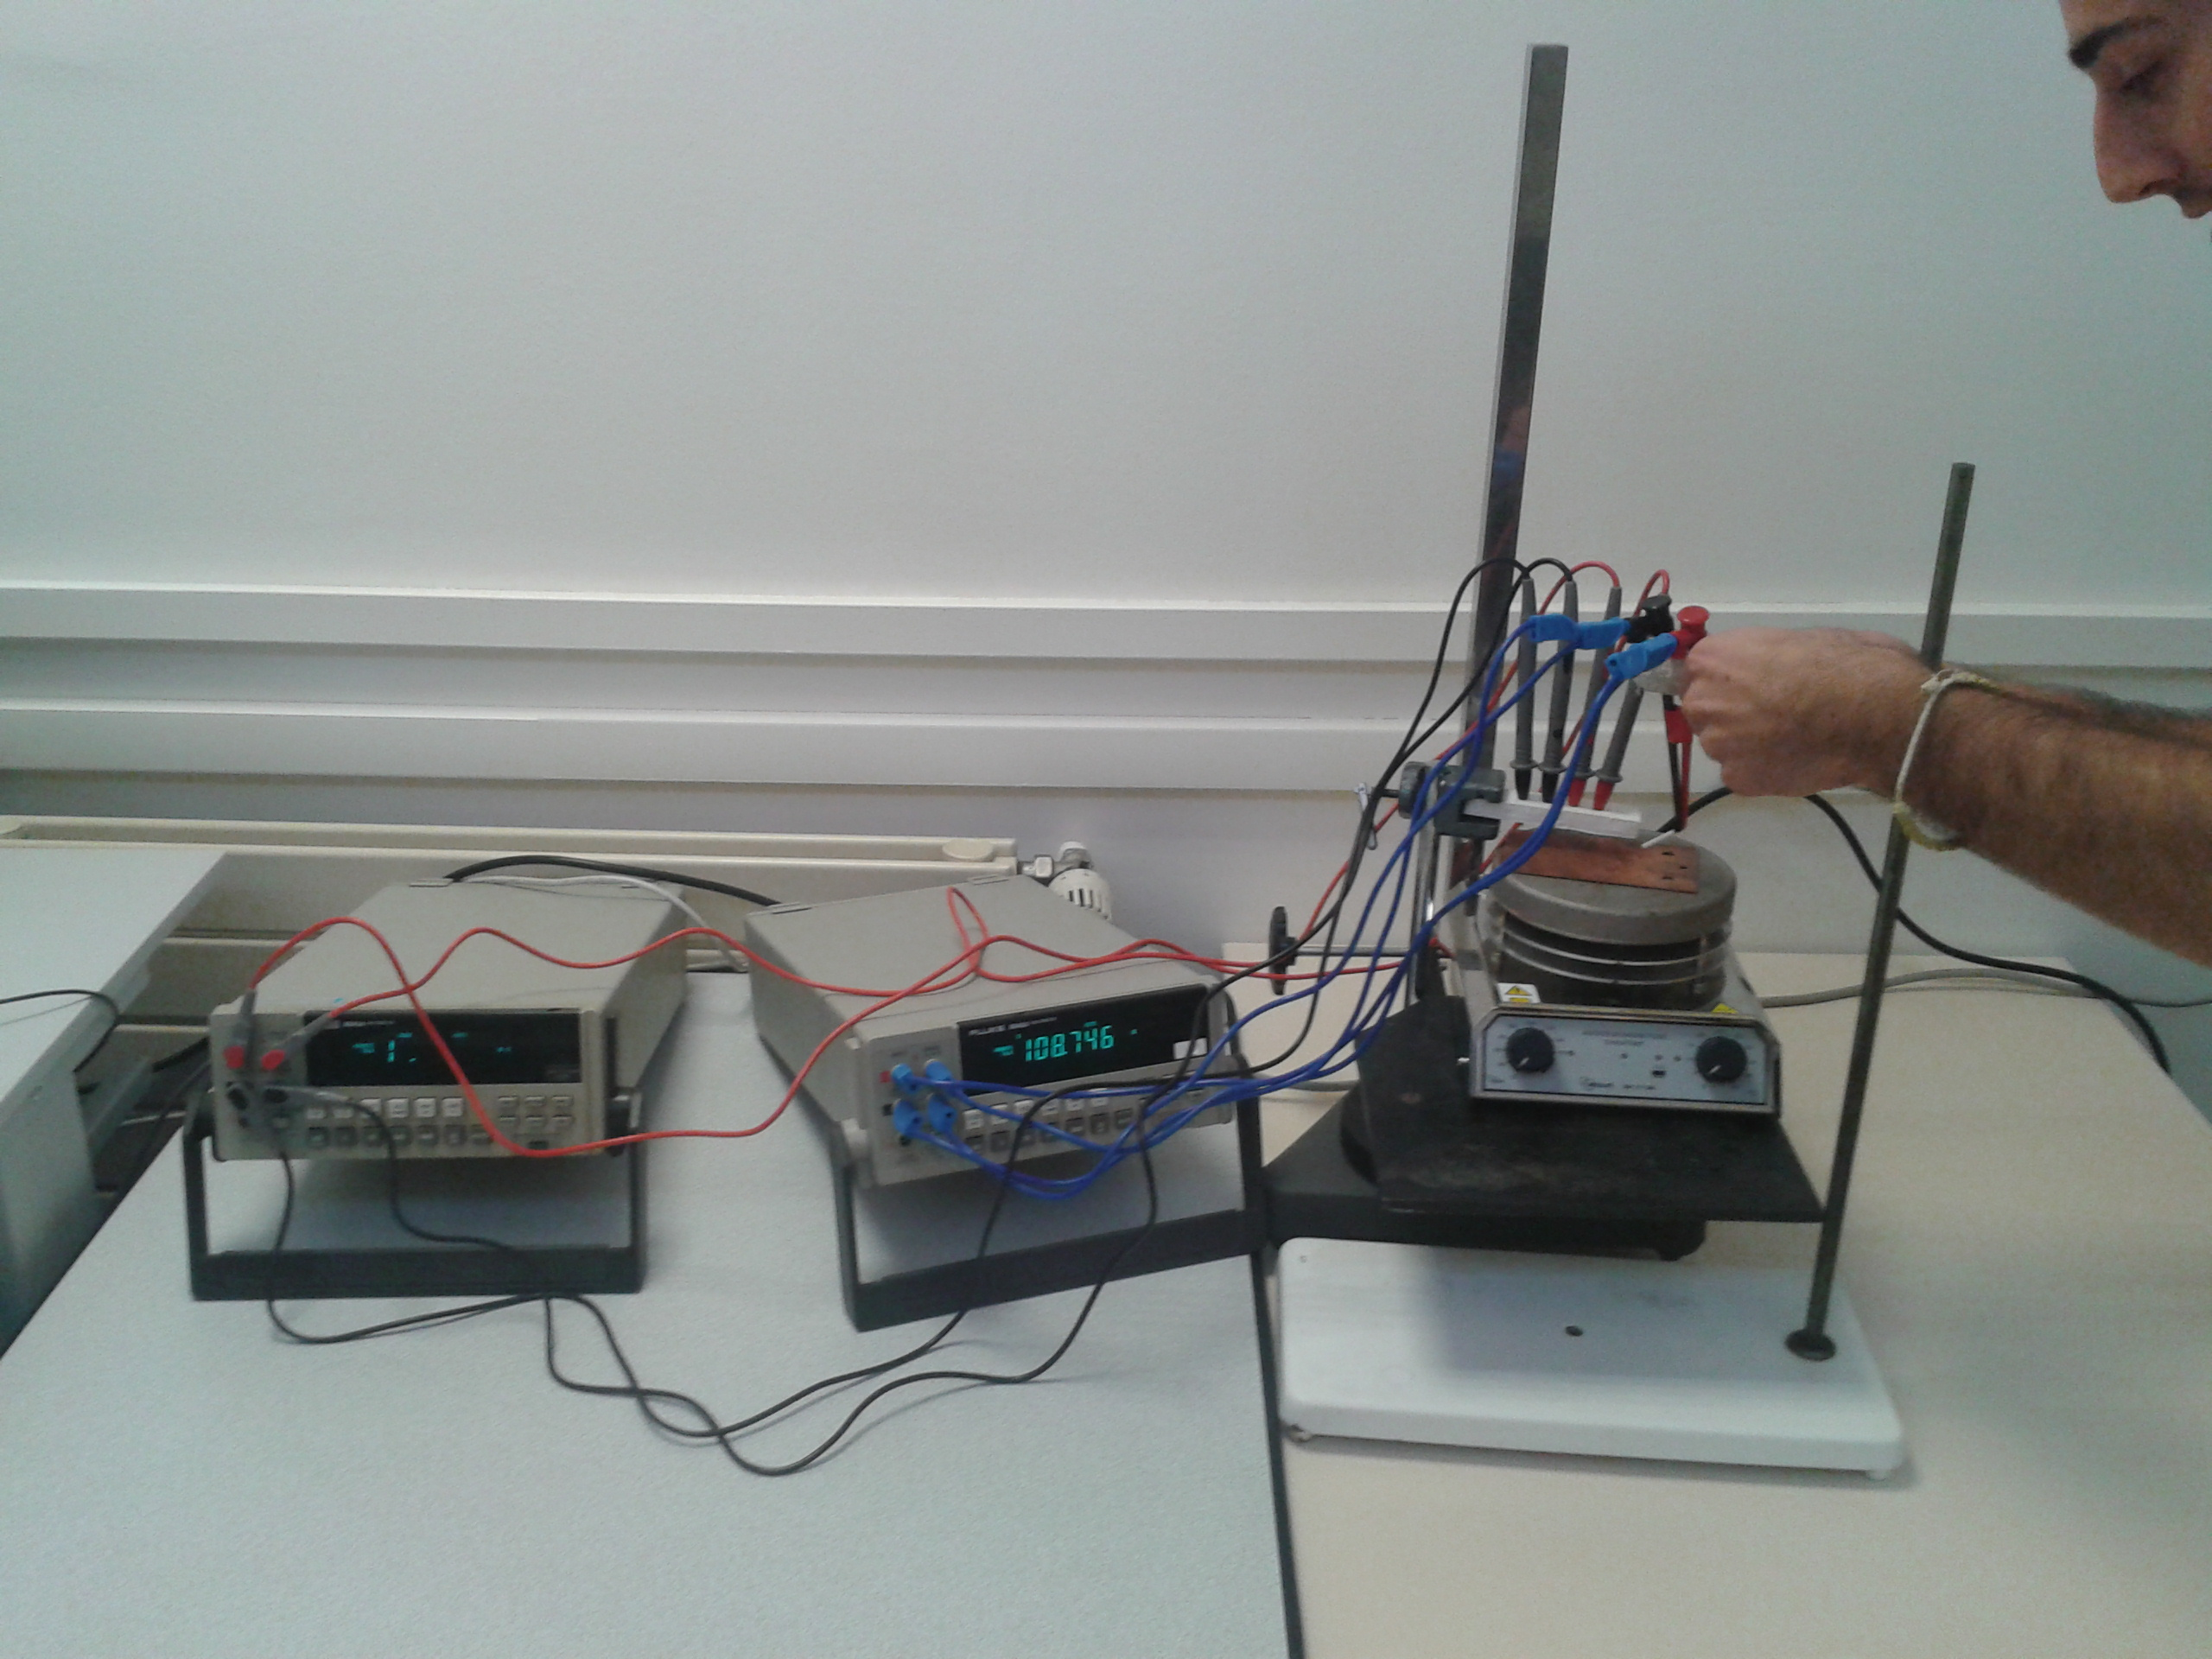
\includegraphics[width=12cm]{./images/photo1.jpg}
		\caption{Montage général}
		\label{photo1}
	\end{center}
\end{figure}

\newpage

\begin{figure}[!t]
  \begin{center}
		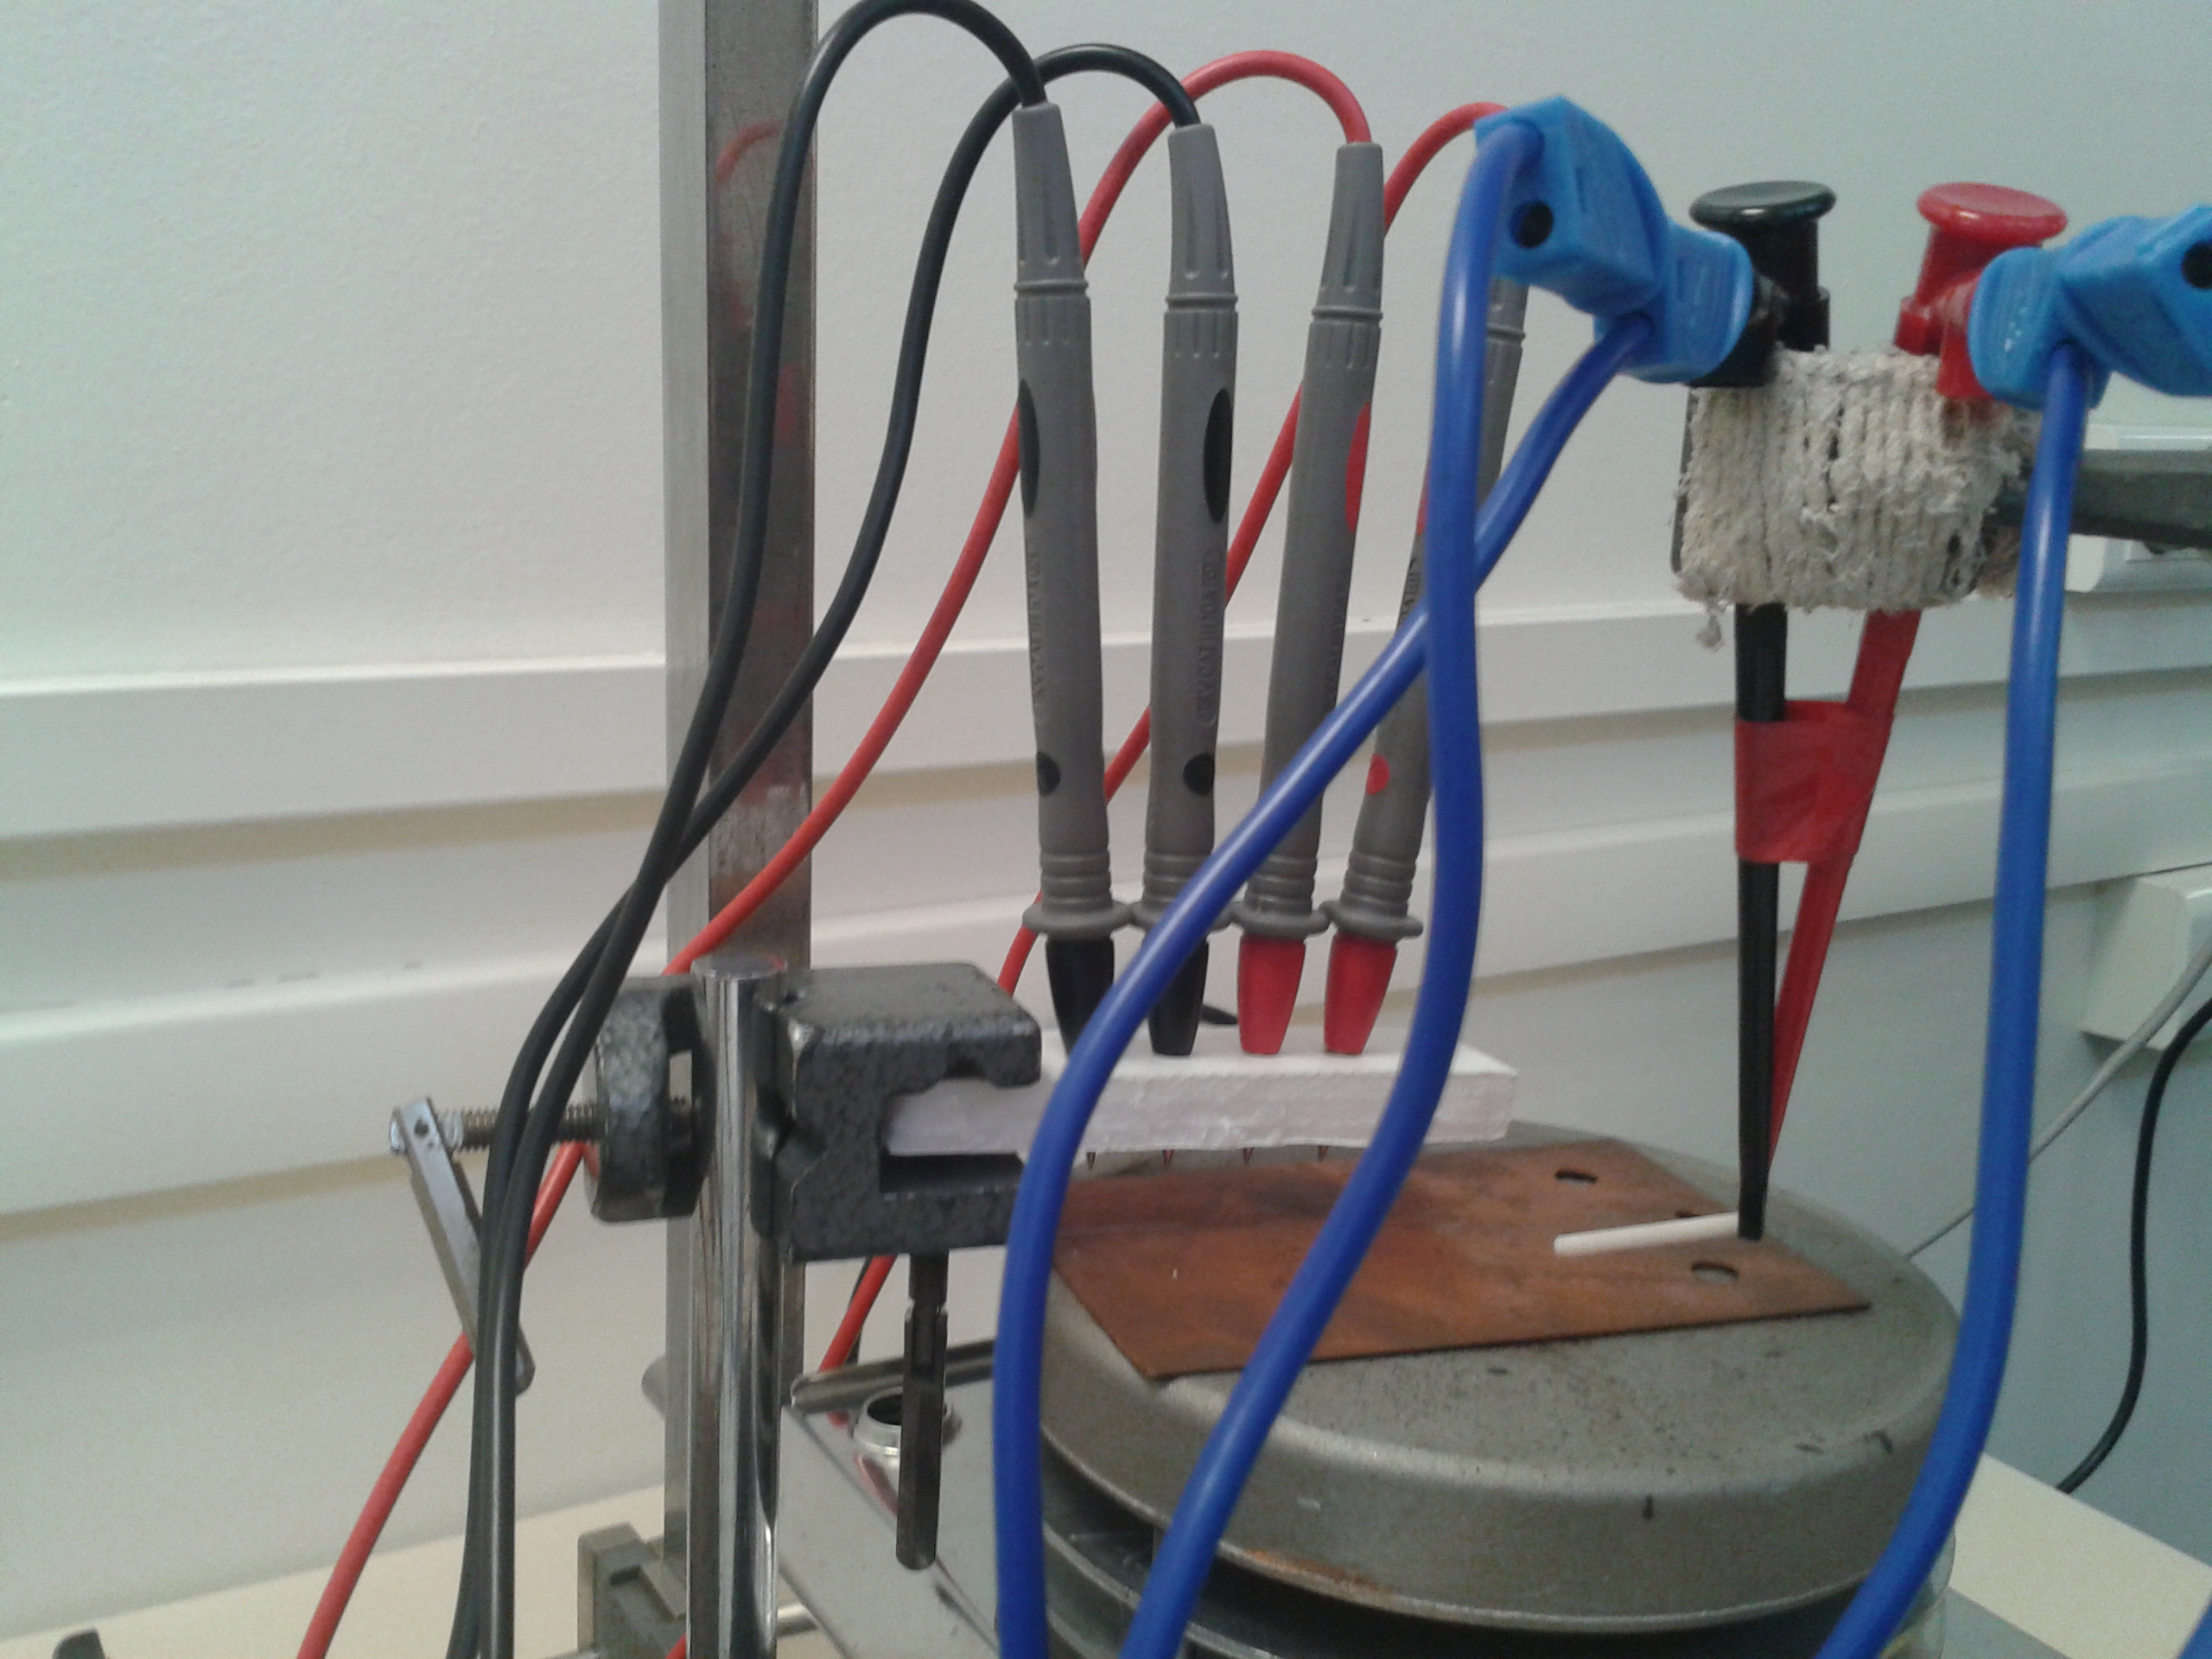
\includegraphics[width=8cm]{./images/photo2.jpg}
		\caption{Gros plan sur les 4 sondes de mesure de résistance (à gauche) et la sonde \emph{Pt100} de température (à droite)}
		\label{photo2}
	\end{center}
\end{figure}
\begin{figure}[h]
  \begin{center}
		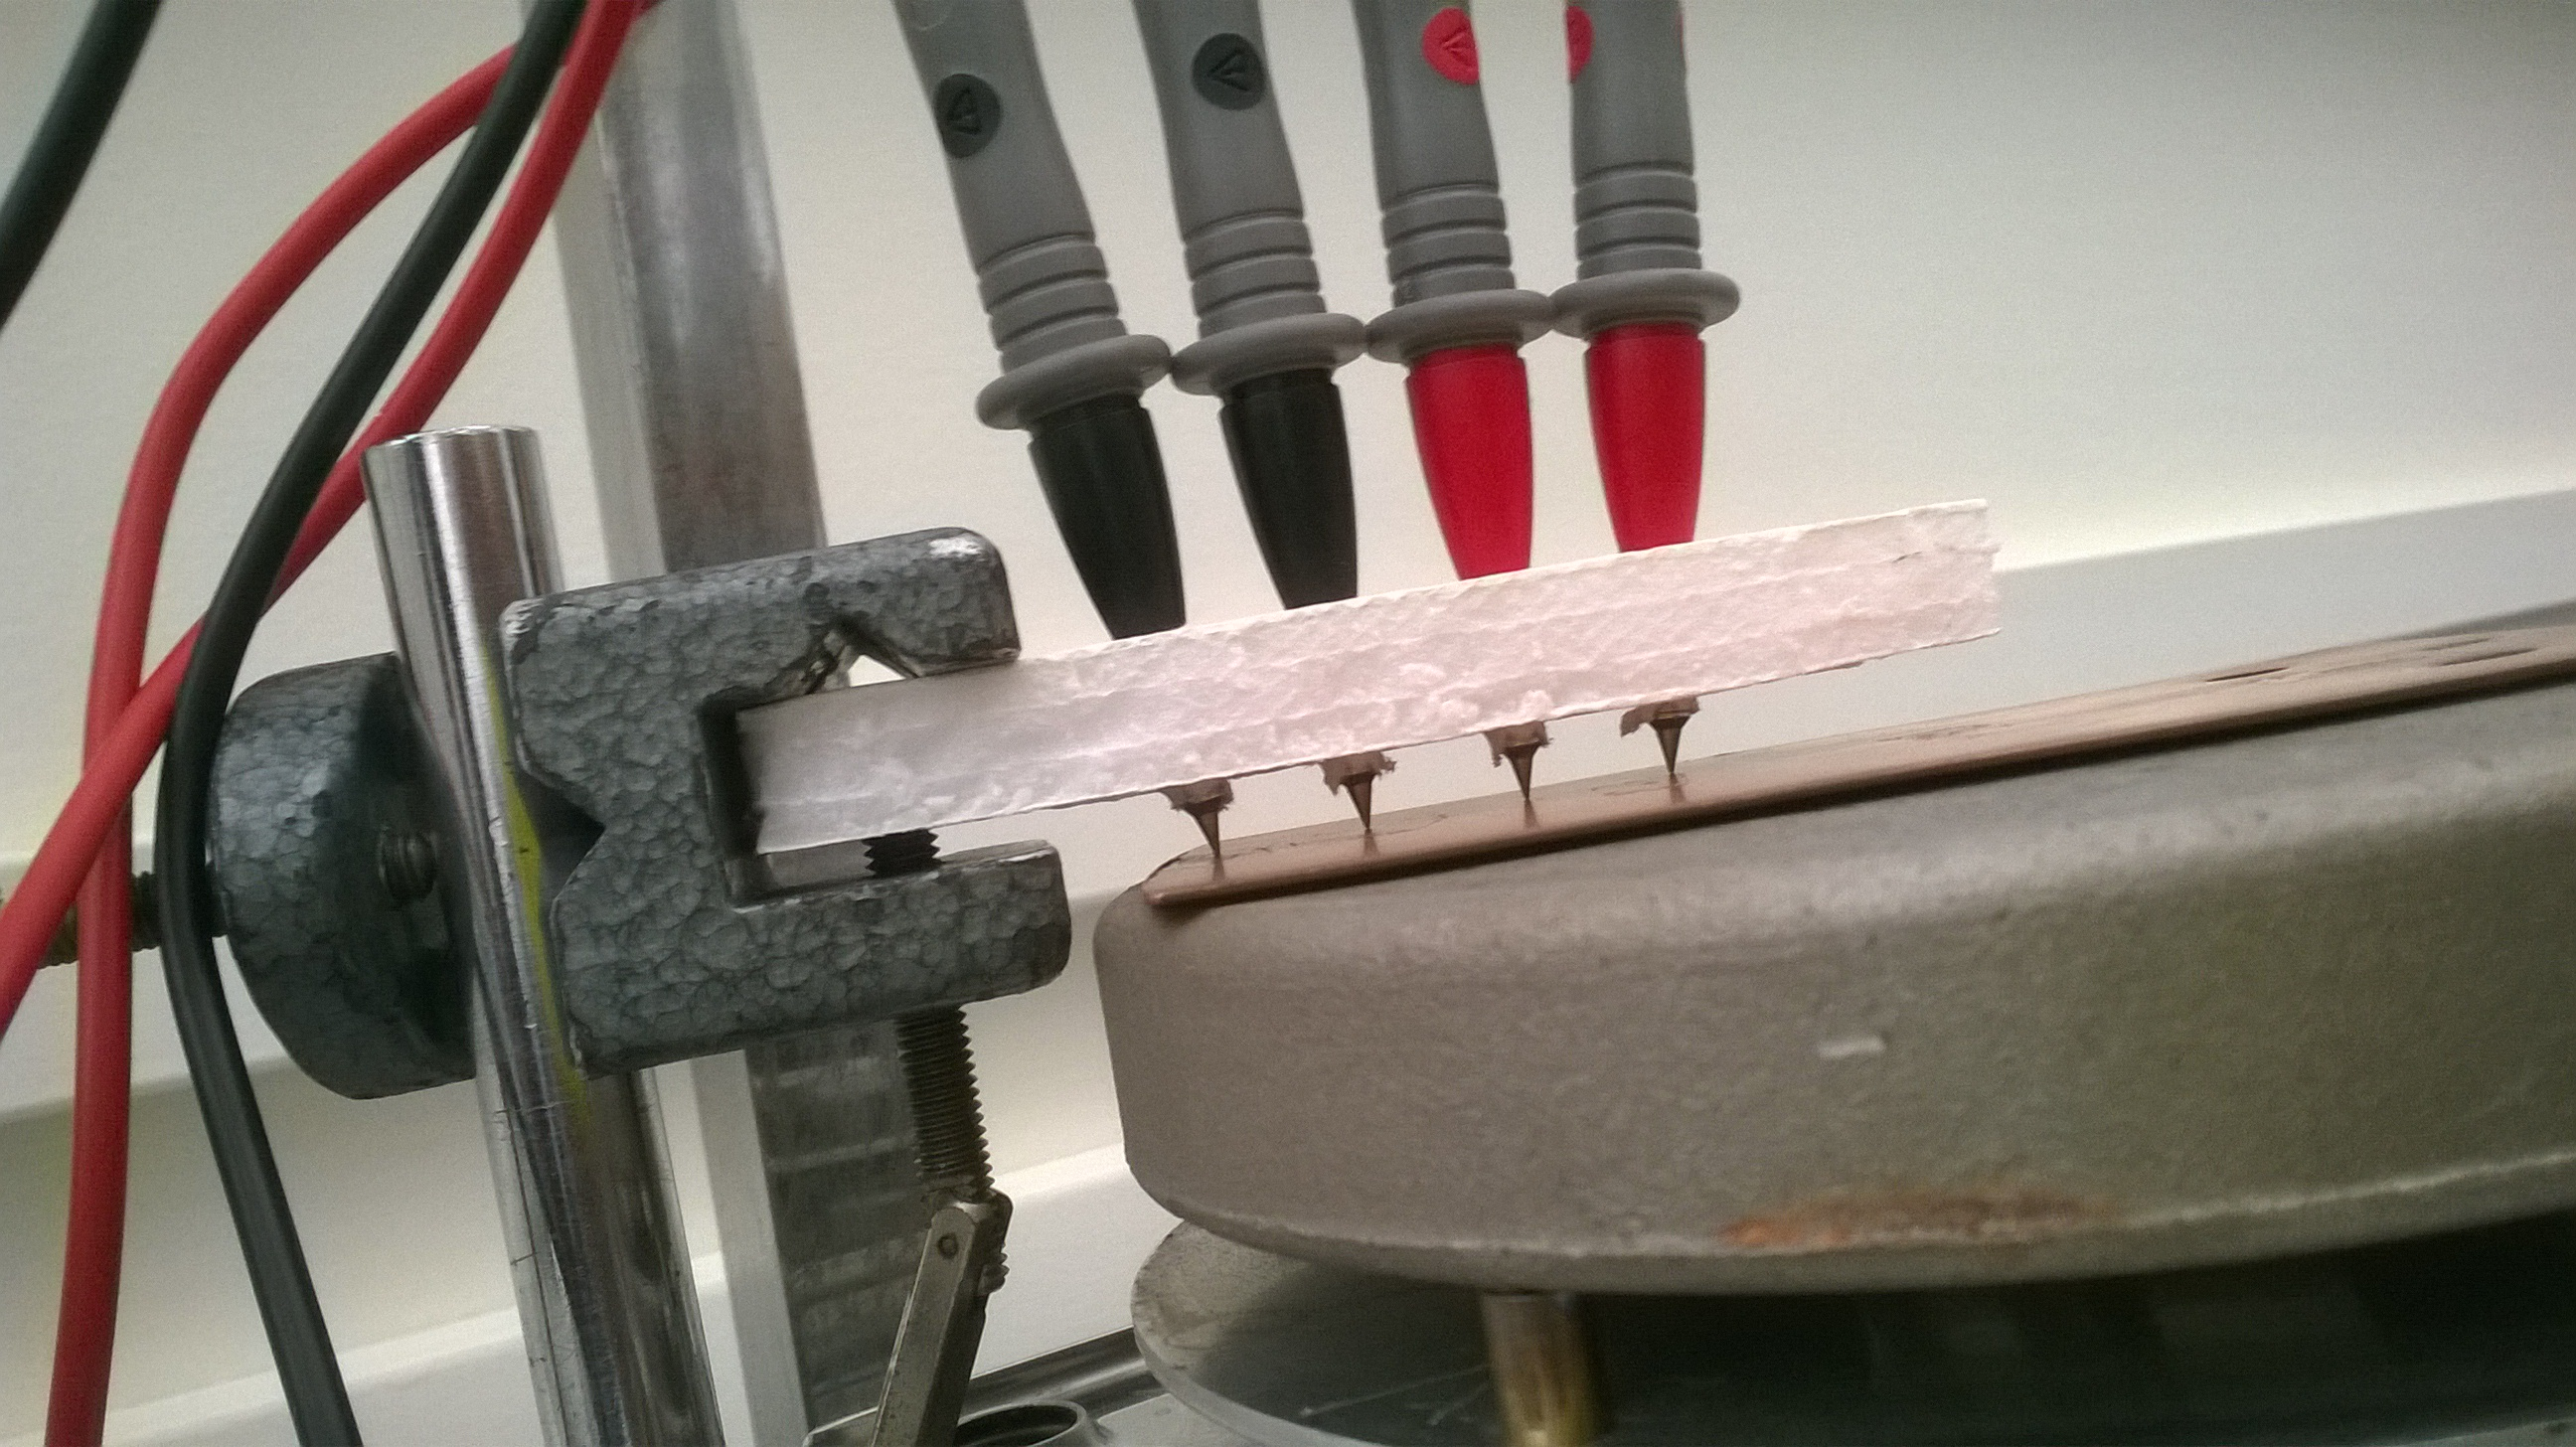
\includegraphics[width=9cm]{./images/photo3.jpg}
		\caption{Les 4 pointes en contact}
		\label{photo3}
	\end{center}
\end{figure}

Sur les 2 photos suivantes : Figures \ref{photo4} et \ref{photo5}, on peut voir le porte-échantillon rempli de billes de verre, et dans lequel est inséré la sonde de température, ce montage étant utilisé dans le cas du refroidissement à l'azote liquide (on verse l'azote dans ce porte-échantillon adapté à ce type de manipulations à très basse température).

\newpage

\begin{figure}[!t]
  \begin{center}
		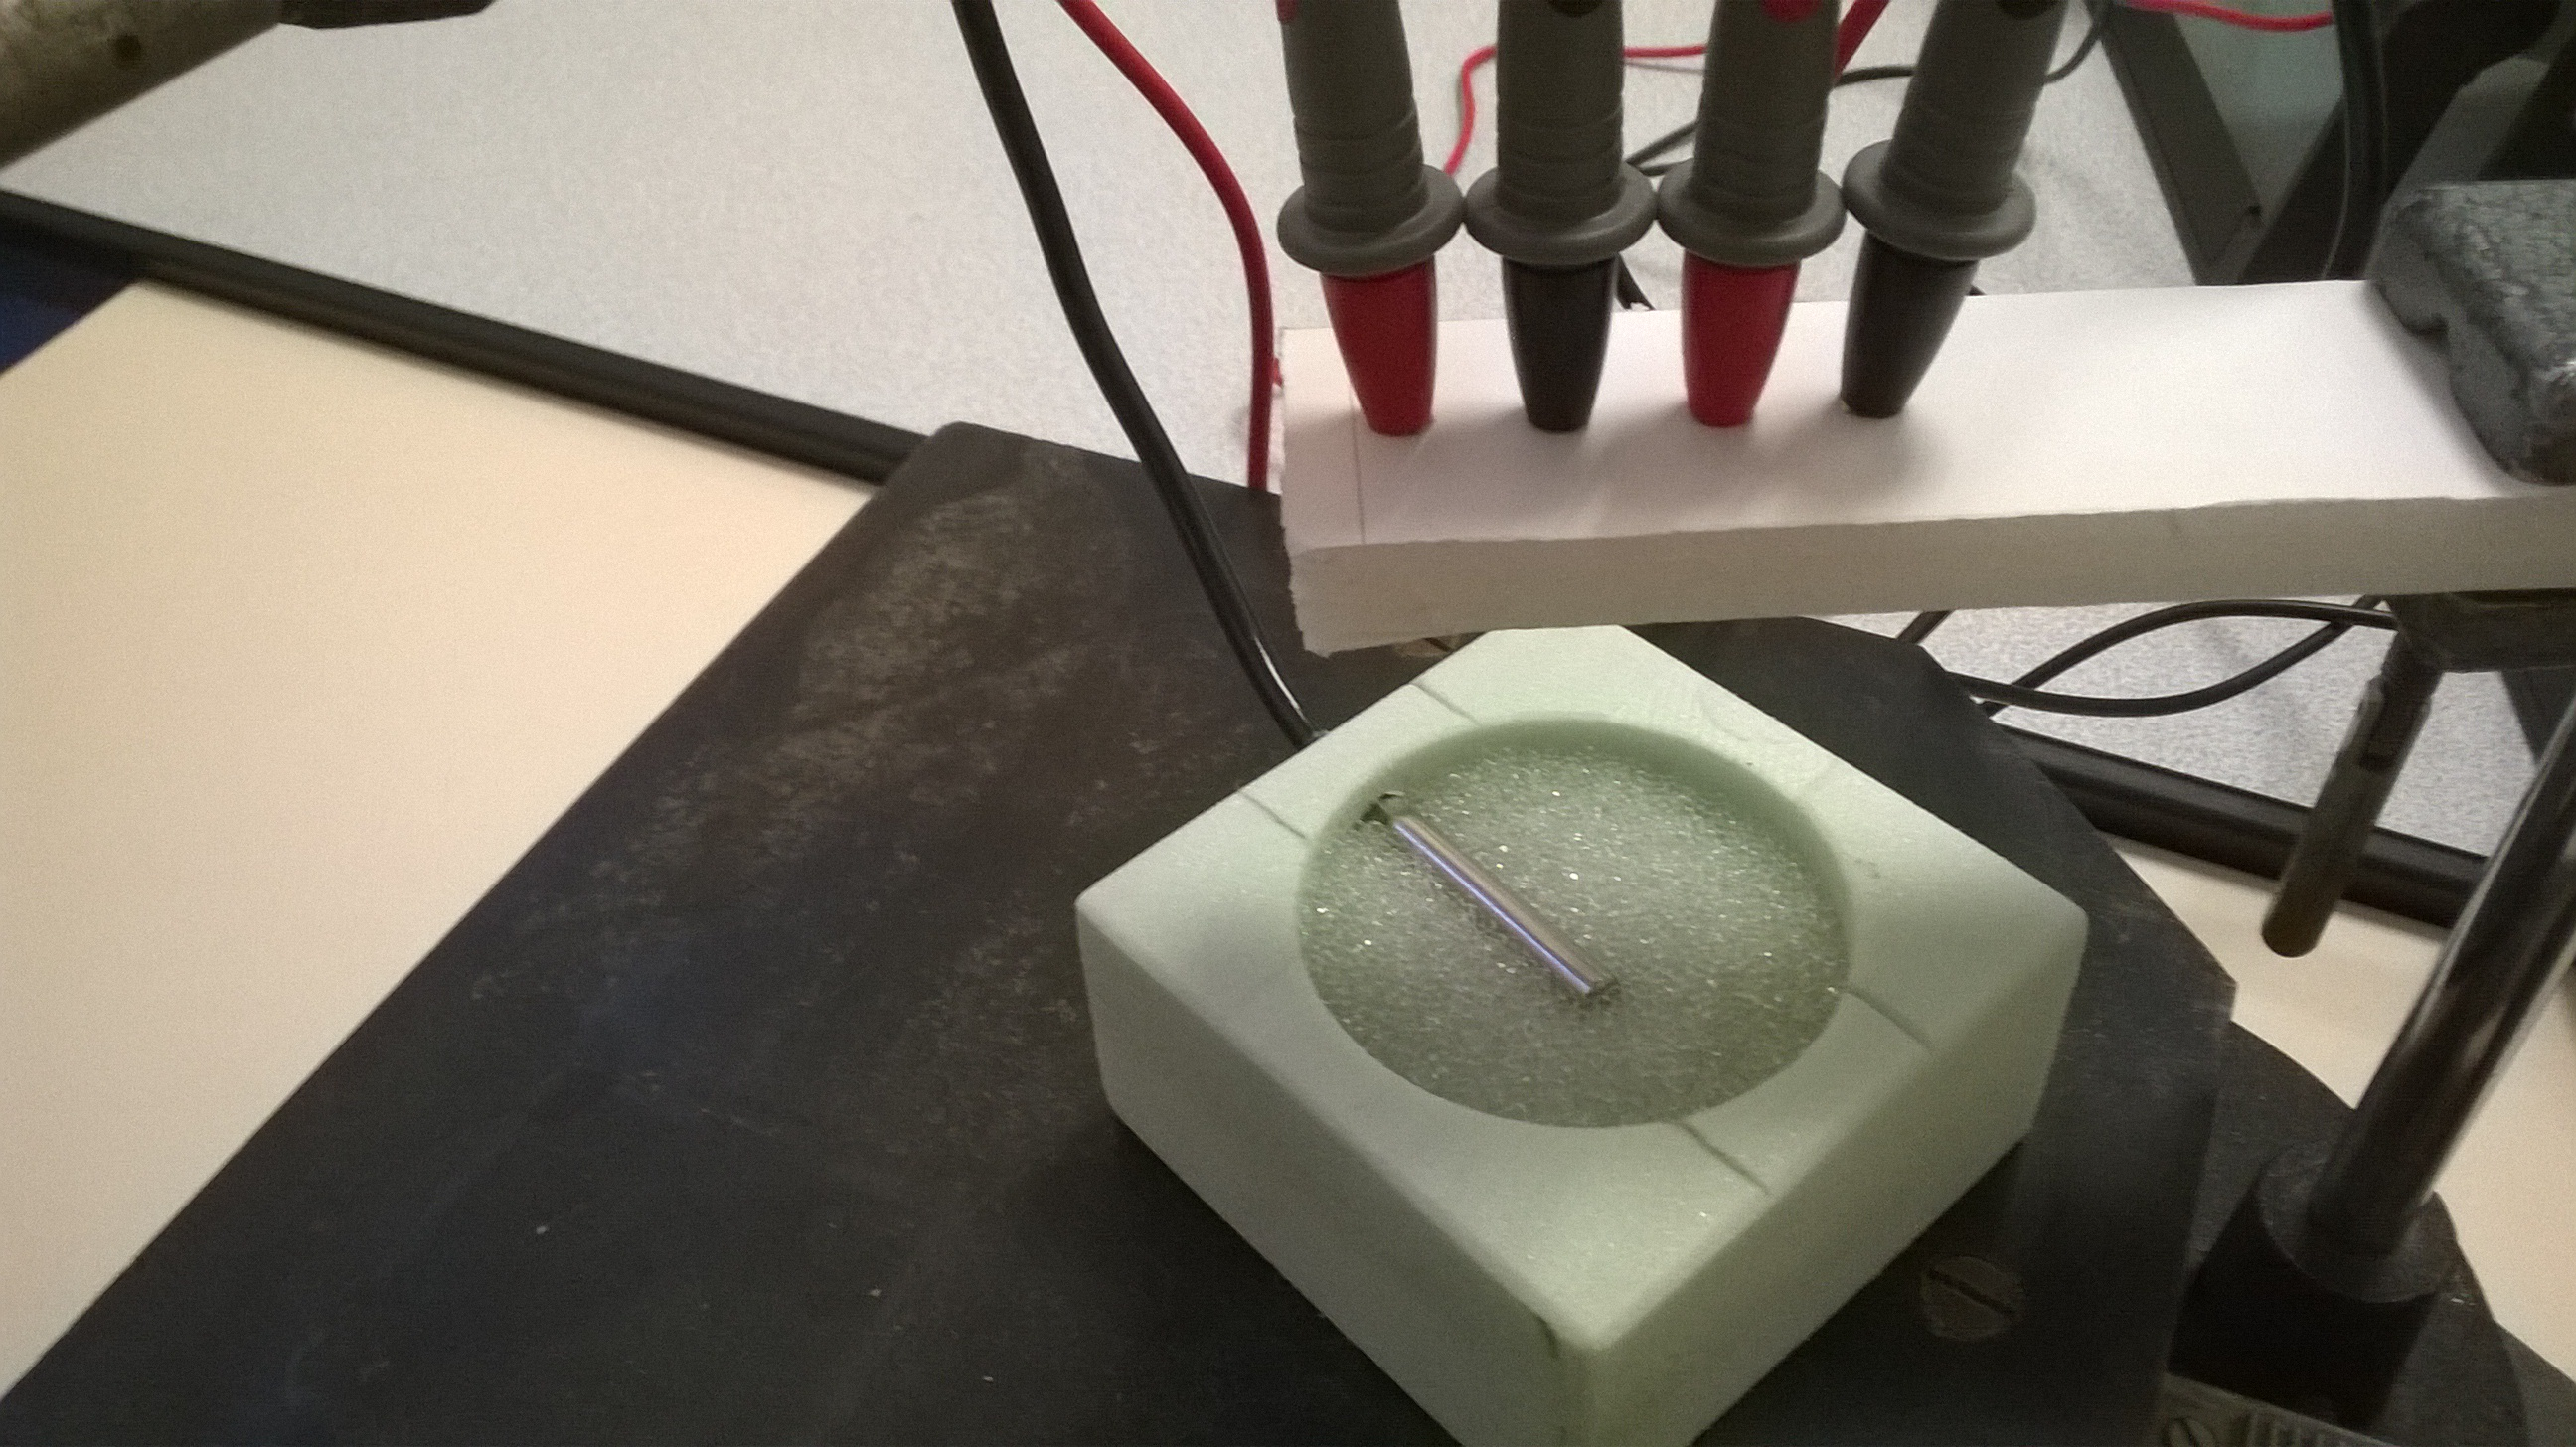
\includegraphics[width=7cm]{./images/photo4.jpg}
		\caption{Porte-échantillon pour le refroidissement à l'azote liquide avec une sonde de température insérée sur le côté.}
		\label{photo4}
	\end{center}
\end{figure}

\begin{figure}
  \begin{center}
		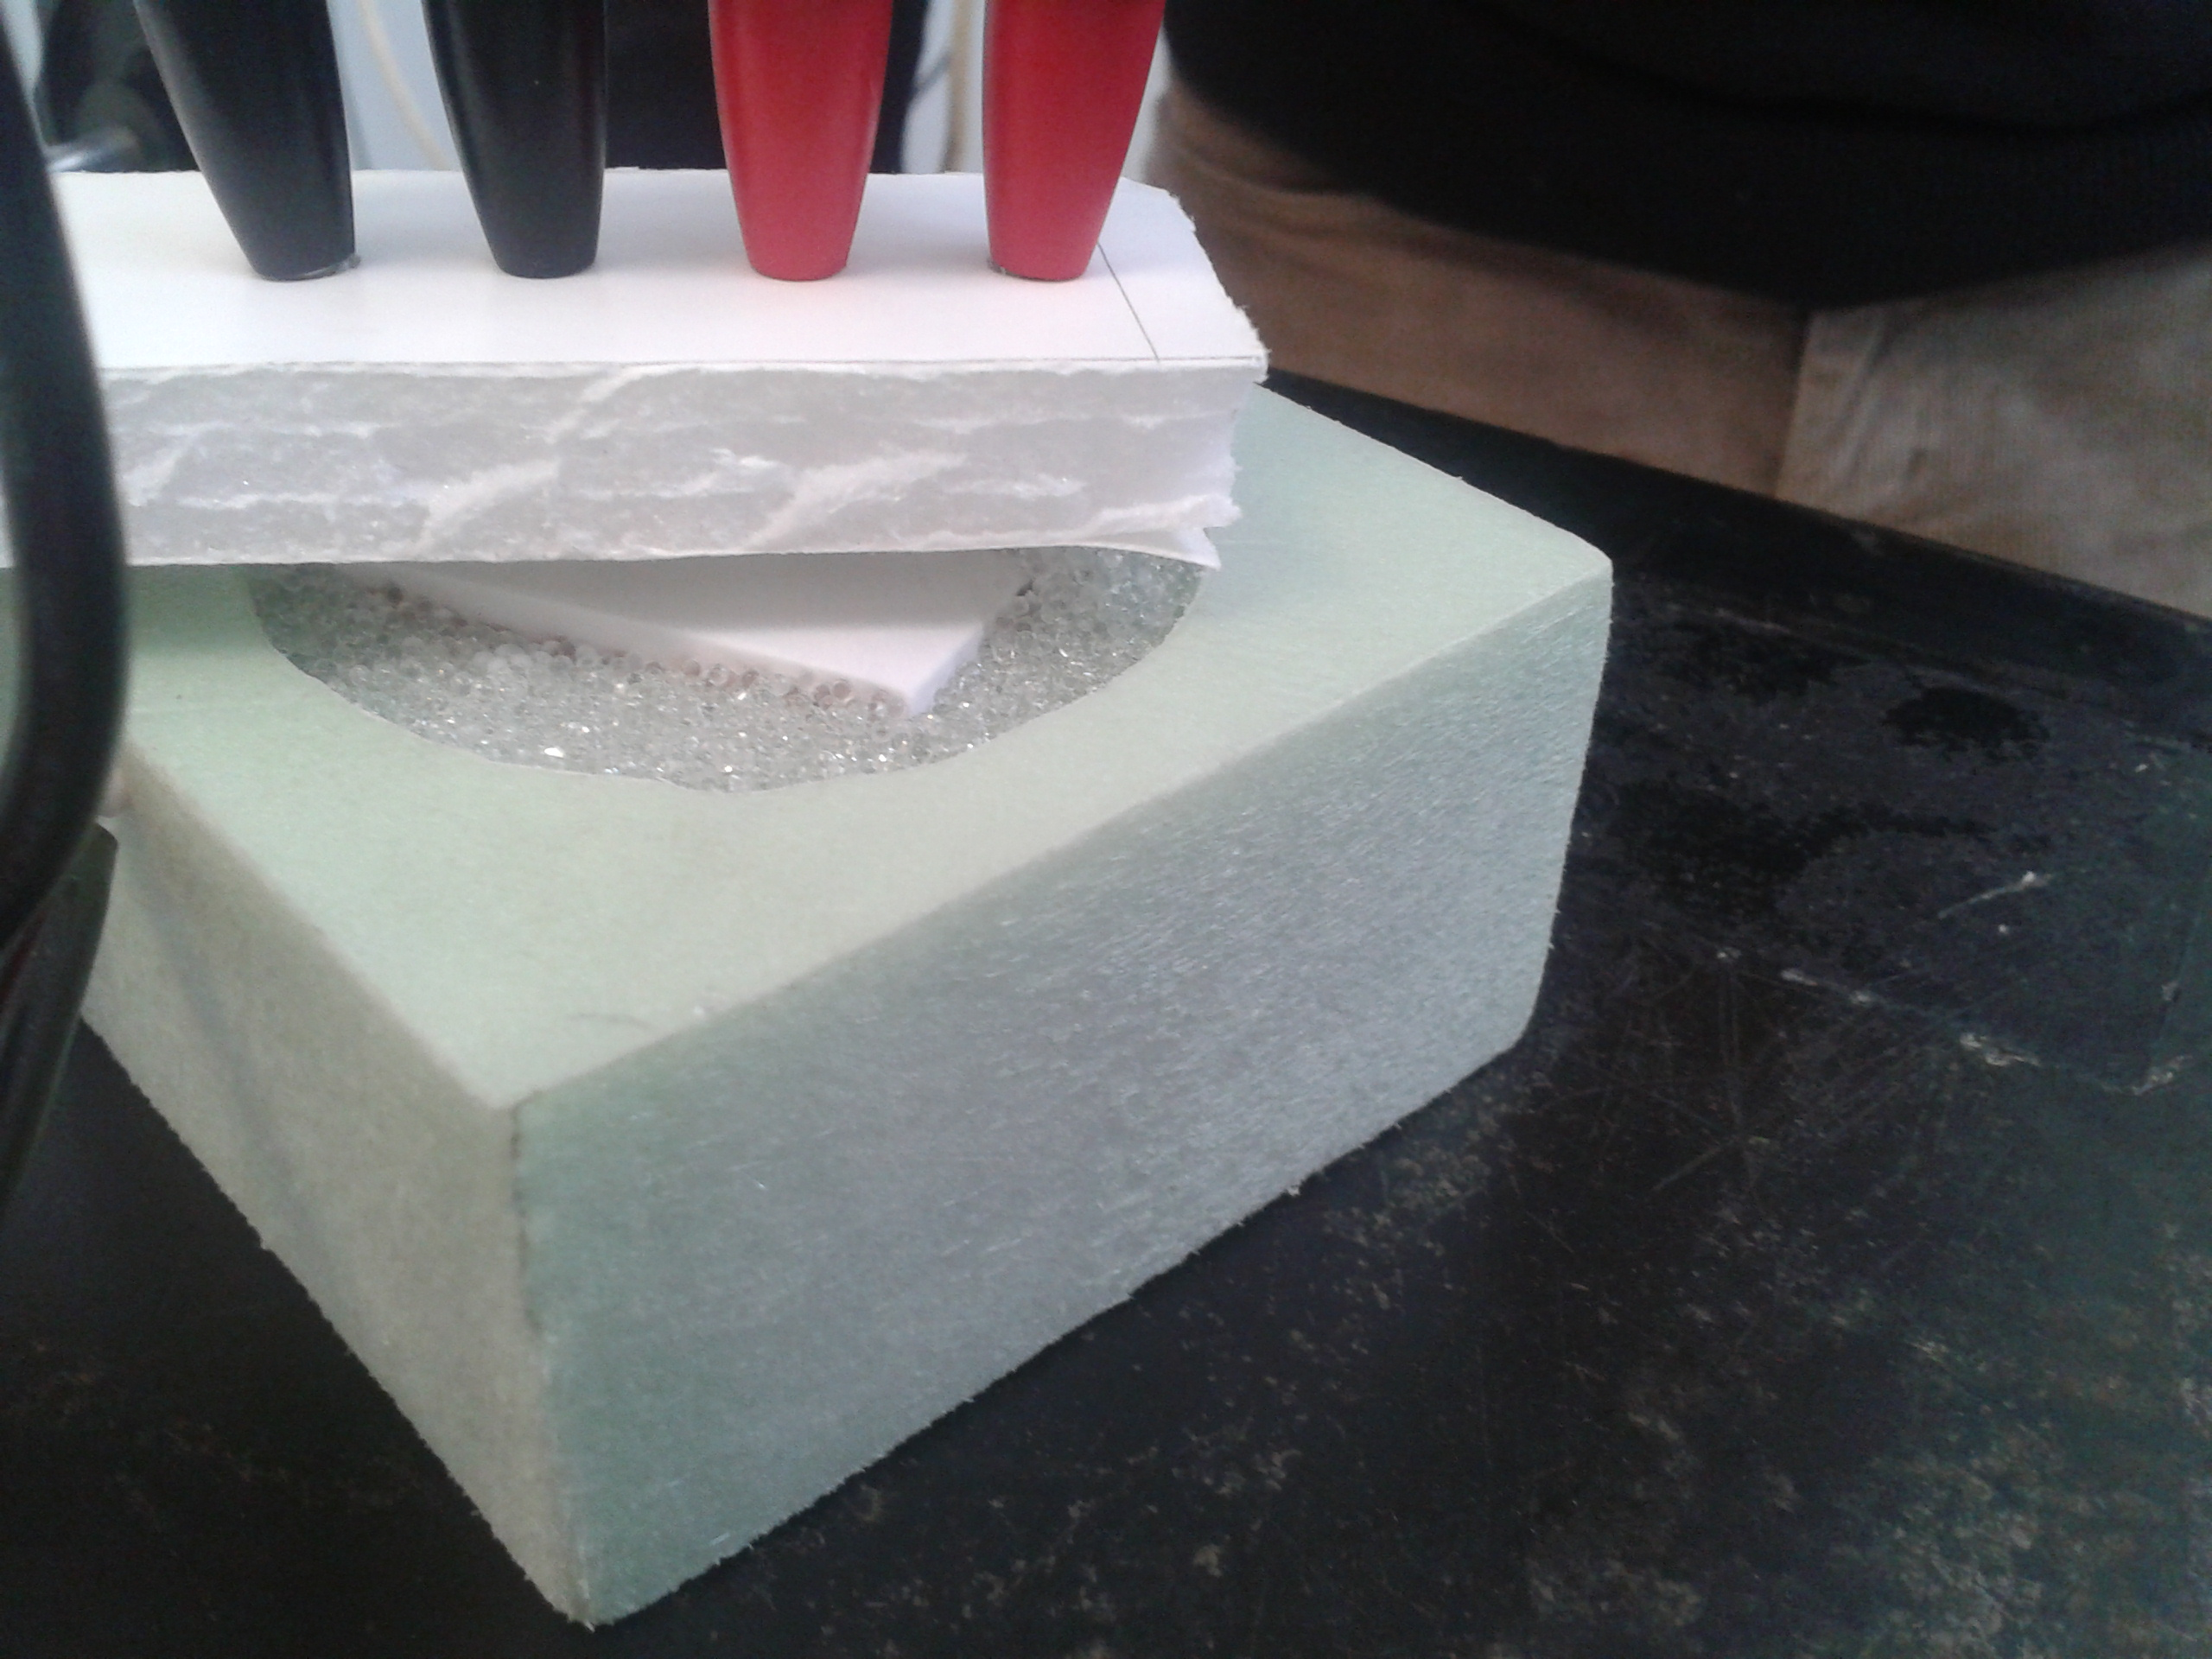
\includegraphics[width=7cm]{./images/photo5.jpg}
		\caption{Les 4 pointes en contact au cours d'une mesure avec refroidissement à l'azote liquide (ici, il s'agit d'un essai avec une petite plaque de cuivre).}
		\label{photo5}
	\end{center}
\end{figure}

Voici enfin une photo du montage à effet Hall [Figure \ref{photo_hall}], que nous avions commencé à préparé, 
mais que nous n'avons malheureusement pas eu le temps de terminer. Nous voulions utiliser un électroaimant, 
on peut aussi observer une source de courant sur la table, ainsi qu'un porte-échantillon à gauche de l'aimant.

\begin{figure}[!t]
  \begin{center}
		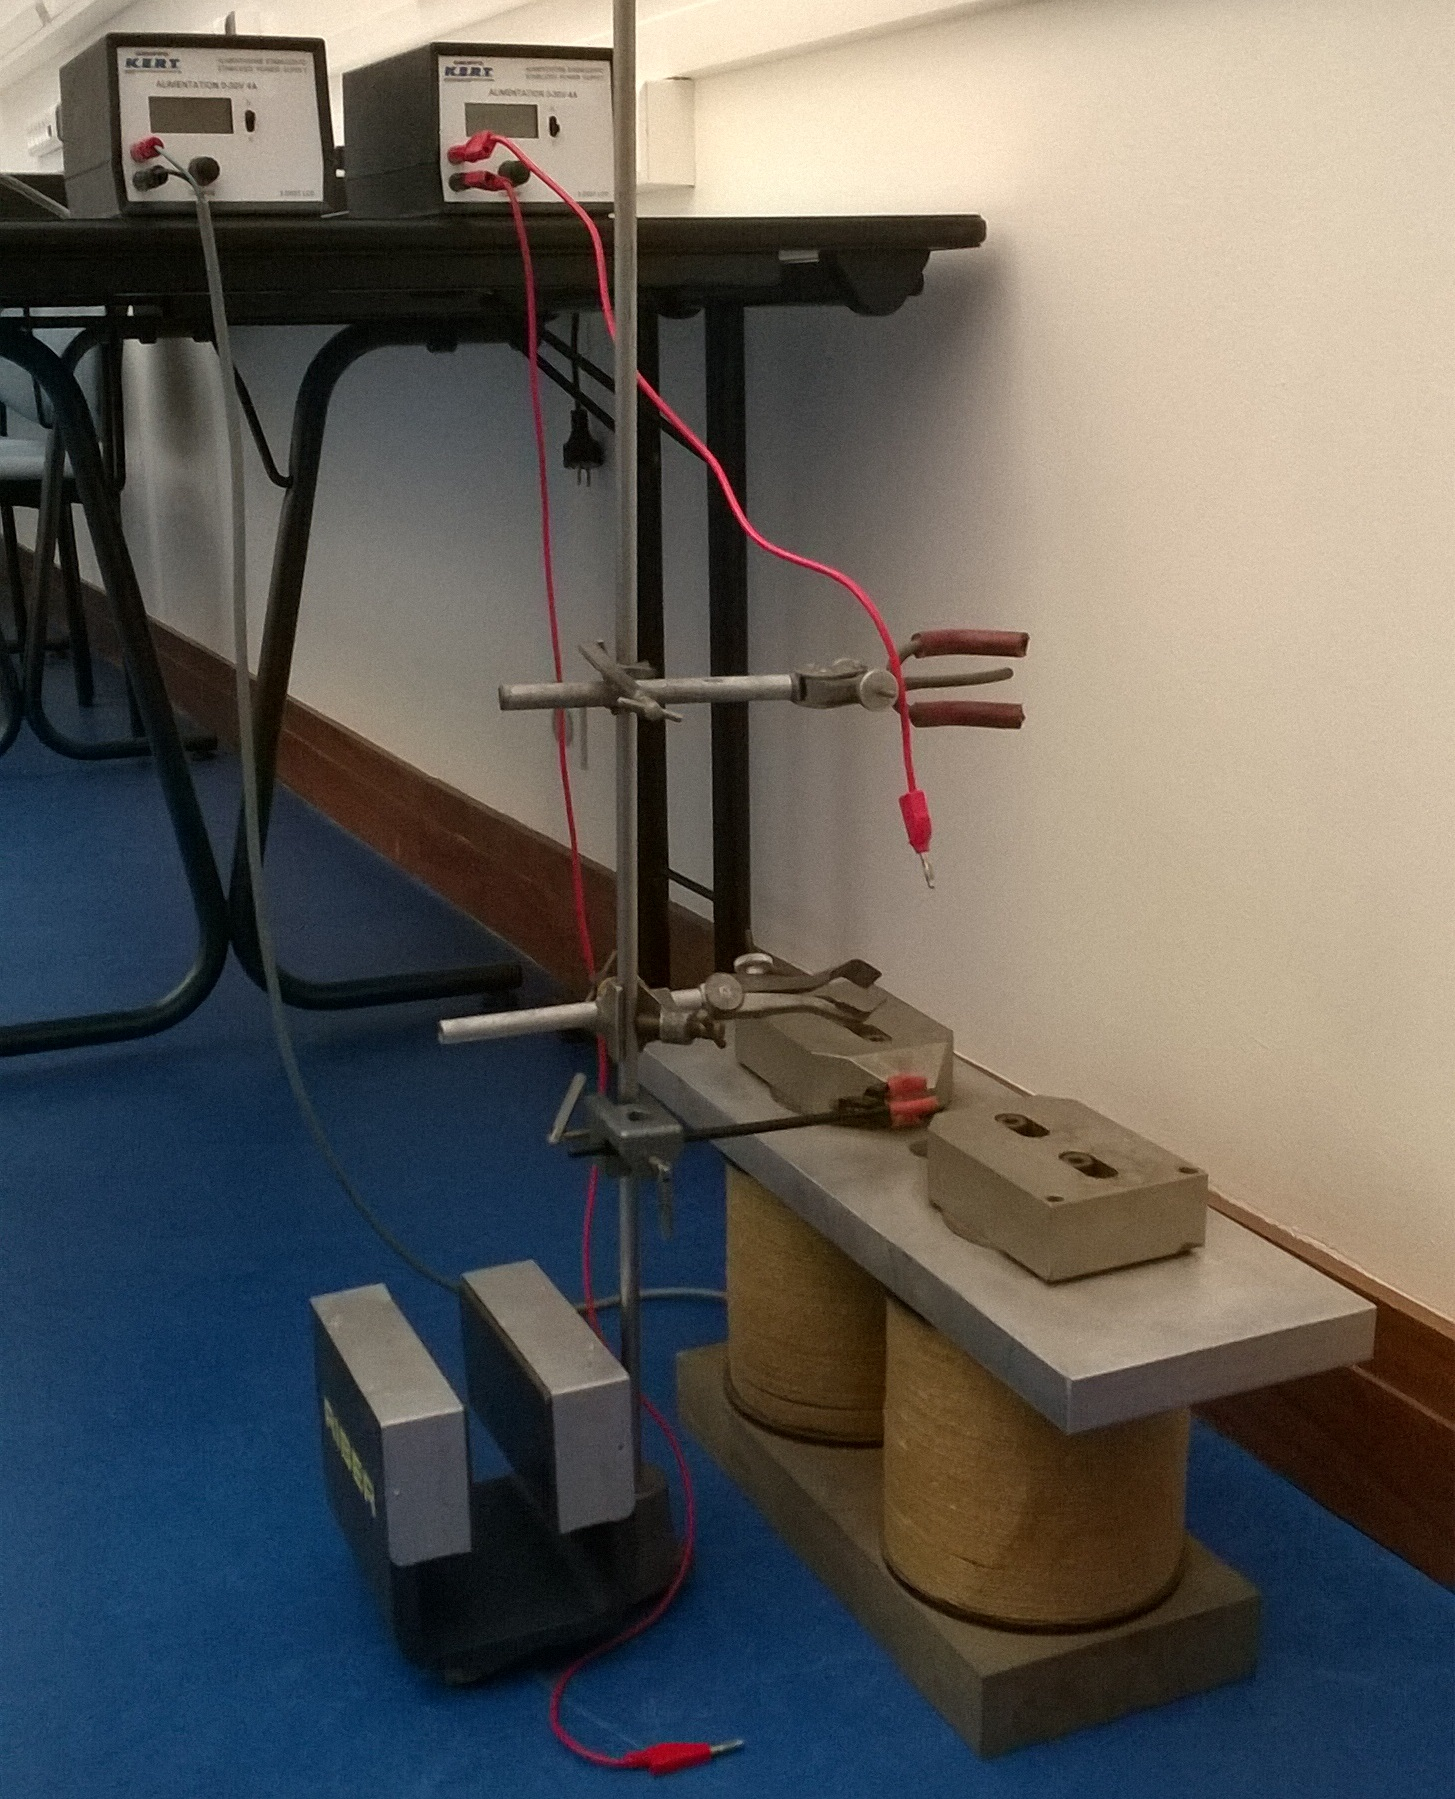
\includegraphics[height=6cm]{./images/photo_hall.jpg}
		\caption{Montage pour la mesure à effet Hall}
		\label{photo_hall}
	\end{center}
\end{figure}

\newpage

\subsection{Conditions expérimentales}
Nous avons utilisé Labview pour réaliser les acquisitions des deux résistances mesurées.
Nous avons simplement posé la plaque de cuivre sur une plaque chauffante et mesuré sa résistance en fonction de la température en 4 pointes, entre 25\celsius{} et 205\celsius{}.


Pour le silicium, nous voulions détecter un palier de conductivité (car il s'agissait d'échantillons dopés), et nous savions que ce palier risquait de se trouver à une température inférieure ou égale à la température ambiante.
Donc, pour pouvoir étudier ce palier, nous avons dû baisser fortement la température et nous avons utilisé de l'azote liquide pour cela.
Nous avons également placé des billes de verre dans notre porte-échantillon pour augmenter l'inertie thermique du montage et nous permettre d'avoir une montée en température relativement lente.
La sonde de température a été insérée dans le porte-échantillon par un trou percé sur le côté (voir Figure \ref{photo4}). De cette façon, elle peut être en contact avec silicium et être entourée par les billes de verre.
De ce fait, elle mesure bien mieux la température du silicium que si on l'avait simplement posée sur l'échantillon.


\paragraph{Pourquoi une mesure 4 pointes (et pas tout simplement 2) ?}
La mesure 4 pointes consiste à injecter un courant avec deux pointes et à mesurer une tension avec deux autres placées entre les deux premières.
Cette méthode permet de s'affranchir des résistances des fils et des résistances de contact.
Elle est donc particulièrement utile pour mesurer des résistances de l'ordre de l'$\Omega$ ou inférieures, car c'est l'ordre de grandeur des résistances parasites.
Par contre, elle est peu utile pour les hautes résistances (plusieurs k$\Omega$, M$\Omega$), donc nous aurions mesuré en 2 pointes pour un isolant par exemple.


\paragraph{Principe et étalonnage de la sonde}
Nous avons étalonné la sonde Pt en deux étapes :

\begin{itemize}
  \item en la plaçant dans de l'eau que nous avons fait bouillir, nous avons pu mesurer la résistance de la sonde à une température de 100\celsius{}.
  \item en la plaçant ensuite dans de l'eau pleine de glaçons, nous avons fait la même chose pour 0\celsius{}.
\end{itemize}

La résistance du platine augmente très linéairement avec la température, c'est une propriété de ce matériau.
On obtient alors la caratéristique R(T) : en mesurant la résistance du Platine, on peut en déduire sa température (donc idéalement la température de l'échantillon).


\paragraph{Interfaçage grâce à Labview}
L'utilisation de l'outil informatique pour mener à bien l'expérience était prévu pour cet AE et en constituait une des principales caractéristiques. En effet notre encadrant nous avait fortement recommandé d'automatiser les mesures pour faciliter la prise de données tout en gagnant en savoir-faire expérimental. L'outil de prédilection pour ce type de mesure est le logiciel \emph{Labview} qui permet de réaliser l'acquisition et le traitement des données. Nous avons donc décidé d'utiliser ce logiciel. Le but était de pouvoir contrôler les deux multimètres avec l'ordinateur. La prise de données par voie informatique comporte trois volets que nous avons dû nous approprier successivement : 

\begin{enumerate}
\item la connexion des appareils à l'ordinateur, 
\item leur reconnaissance par ce dernier, 
\item et la réalisation du code LabView. 
\end{enumerate}

La première étape a été réalisée grâce à deux câbles \emph{smart488}, mais le laboratoire n'ayant qu'un seul câble de ce type, nous avons dû en commander en deuxième.
Ces câbles permettent le passage d'une sortie GPIB à une sortie USB et possèdent un contrôleur intégré. 
C'est ce contrôleur qu'il a fallu régler, grâce à un logiciel dédié, pour pouvoir détecter les deux multimètres 
via l'ordinateur. Nous avons aussi utilisé le logiciel NI-Max pour vérifier la compatibilité de ces éléments avec Labview. 

Après cela nous avons entamé l'étape d'écriture du code graphique Labview [Figure \ref{code_labview}]. Ce code devait nous permettre d'acquérir 
simultanément, et dans le temps, les signaux des deux multimètres, qui correspondent à la température de la sonde 
et à la résistance de l'échantillon. L'acquisition se fait pendant un laps de temps prédéfini. Les résultats obtenus sont présentés sous forme de tableau de nombres dans un fichier texte qui peut être lisible par un logiciel comme gnuplot ou Excel.
Nous avons en effet utilisé gnuplot par la suite pour tracer nos courbes.

\begin{figure}[!t]
  \begin{center}
		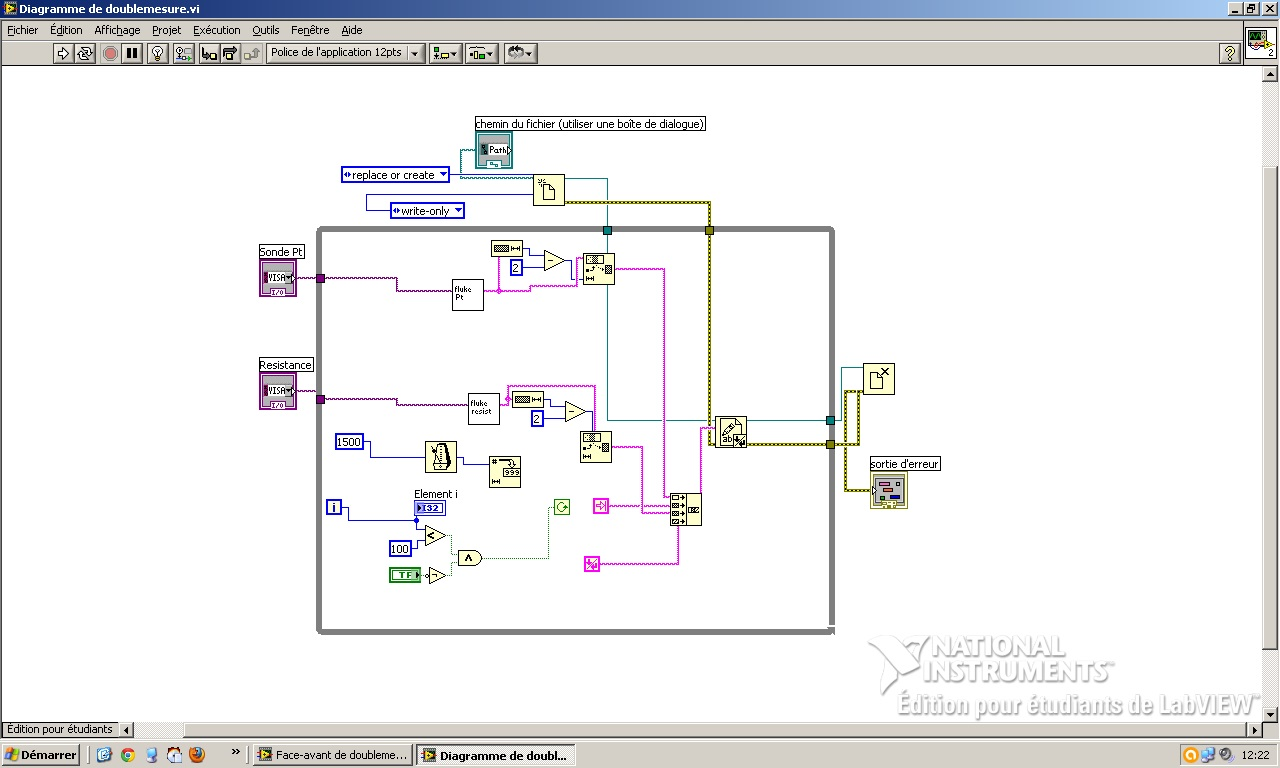
\includegraphics[height=6cm]{./images/labview.jpg}
		\caption{Code de notre programme Labview}
		\label{code_labview}
	\end{center}
\end{figure}

\newpage

\subsection{Difficultés expérimentales}
Deux principales difficultés expérimentales se sont posées lors de cette activité expérimentale.
Tout d'abord, il y a eu le problème de l'automatisation des résultats et de l'interfaçage avec l'ordinateur.
Nous avons eu du mal à réaliser chacune des trois étapes liées à l'automatisation des mesures, mais plus particulièrement 
la détection des instruments par l'ordinateur, ceci mettant en jeu différents composants tels que le 
multimètre, le câble smart488 et Labview.

\bigskip

D'autre part, le contact entre les électrodes et l'échantillon s'avéra bien plus délicat que prévu. 
En effet l'utilisation du montage à quatre pointes oblige à avoir quatre contacts stables.

Nous avons d'abord utilisé de la laque d'argent pour réaliser les contacts, mais cela ne s'est pas avéré facile à mettre en place ni très efficace.
Nous avons donc implémenté le montage tel qu'il apparaît dans les photos [Figures \ref{photo1} à \ref{photo5}].

Le premier essai sur le cuivre donna des résultats 
très cohérents mais les essais sur les échantillons de silicium donnaient des valeurs très instables. 
En effet la valeur de la résistance changeait de plusieurs ordres de grandeurs selon la pression exercée sur les 
pointes.

\bigskip

Nous soupçonnons les fils et les pointes d'être a l'origine de ces fluctuations (contacts imparfaits), mais une piste intéressante est l'hétérogénéité de la surface de l'échantillon de silicium. 
En effet le silicium au contact de l'air s'oxyde et on obtient une couche de SiO$_2$ à la surface de l'échantillon. 
La variation de la résistance selon la pression exercée sur les pointes peut donc provenir du fait que la pointe 
traverse ou pas cette couche.

En effet, lorsque l'on exerce une pression constante on obtient des résultats cohérents avec la nature semiconductrice du silicium comme on pourra le voir dans la section suivante. Une façon d'obtenir cette pression constante et donc un meilleur contact est d'utiliser des pointes à ressorts, fixées solidement au support. Cependant, nous n'avons pas pu nous procurer de tels contacts avant la fin de l'activité et nous avons dû réaliser plusieurs fois la même expérience jusqu'à obtenir une mesure stable.

\subsection{Résultats}
Pour commencer et avant de s'attaquer à une mesure sur un semi-conducteur qui s'annonçait complexe, nous avons testé notre montage avec une mesure sur un conducteur très simple : une plaque de cuivre.

Nous avons posé la plaque de Cu sur une plaque chauffante, et nous avons mesuré sa résistance en 4 pointes pour des températures allant de la température ambiante (environ 20 \celsius{}) à envrion 200 \celsius{}. La sonde Pt100 était posée sur la plaque pour suivre la température, comme on peut le voir sur la Figure \ref{photo2}. Toutes les mesures ont été prises via un interfaçage avec Labview.

\bigskip

Nous avons ainsi observé très logiquement une augmentation de la résistance de la plaque en fonction de la température. On peut observer cette tendance sur la Figure \ref{courbe_cuivre}, sur laquelle une régression linéaire a été effectuée et pour laquelle on obtient un bon coefficient de corrélation : $R > 0.99$.

\begin{figure}[hb]
  \begin{center}
		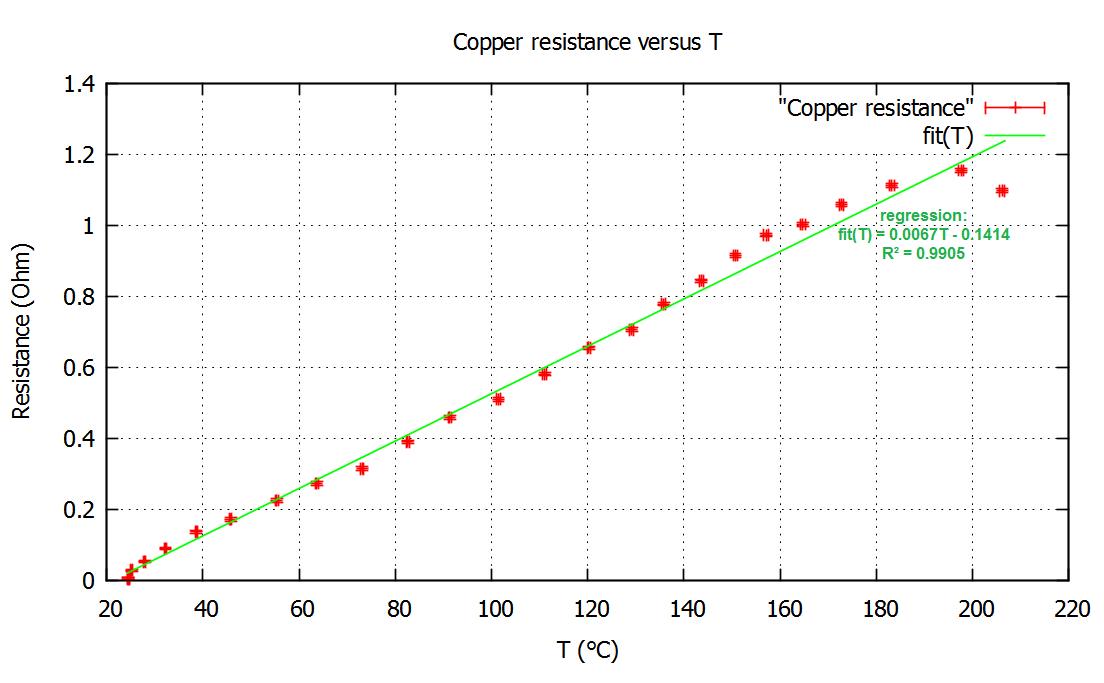
\includegraphics[width=12cm]{./images/Resistance_Cuivre_finale_english.png}
		\caption{Résistance de la plaque de cuivre en fonction de la température. En vert la régression linéaire et ses caractéristiques.}
		\label{courbe_cuivre}
	\end{center}
\end{figure}

\newpage

Ceci est bien en phase avec le modèle de Drude de la conduction électrique, pour lequel la conductivité d'un métal a cette expression (voir \cite{kittel_introduction_1976}) : 
\begin{equation}
	\sigma = \frac{n e^{2} \tau}{m}
\end{equation}
$n$ étant la densité volumique d'électrons, $e$ et $m$ la charge et la masse des électrons, et $\tau$ le temps de vol moyen entre deux collisions d'électrons. Plus la température augmente, plus le taux de collisions entre électrons augmente et donc plus $\tau$ diminue, ainsi $\sigma$ diminue et la résistance de l'échantillon augmente.

\bigskip

Ensuite, nous avons réalisé la mesure pour un wafer de silicium dopé de type N. Il a été placé sur un lit de billes de verre, billes dans lesquelles la sonde de température était placée (voir Figure \ref{photo4}). Là encore, la mesure a été effectuée en 4 pointes et avec l'aide de Labview une première fois (infructueuse), puis sans Labview pour pouvoir mieux contrôler le déroulement de la mesure. Les mesures ont donc été notées à la main. On peut observer les résultats sur la Figure \ref{courbe_silicium}.

\begin{figure}[hb]
  \begin{center}
		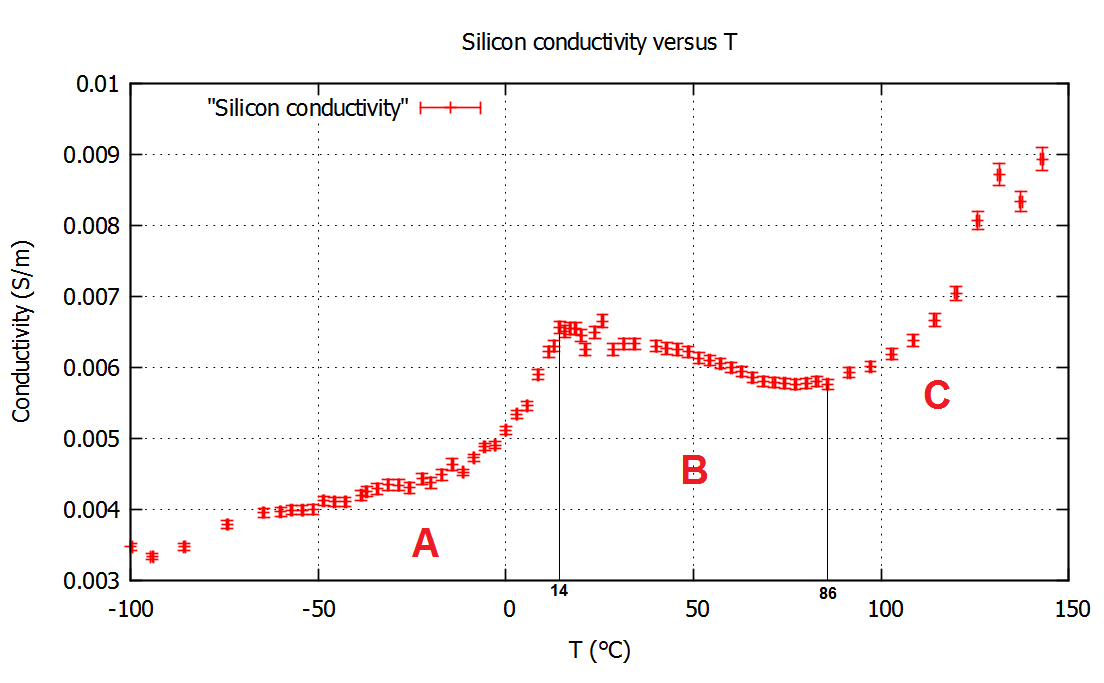
\includegraphics[width=12cm]{./images/Conductivite_Silicium_finale_english.png}
		\caption{Conductivité du wafer de silicium de type N en fonction de la température. Les trois régimes sont notés A, B et C. Le régime A est une croissance en loi d'Arrhénius pour les électrons venant des impuretés. Le régime B est un palier. Le régime C est lui aussi en loi d'Arrhénius, cette fois-ci pour les électrons venant de la bande de valence.}
		\label{courbe_silicium}
	\end{center}
\end{figure}

\newpage

Nous avons bien observé une conductivité croissante avec la température comme prévu, avec un palier aux alentours de [20\celsius{}; 80\celsius{}], ce qui est cohérent avec ce qu'on peut trouver dans \cite{kittel_introduction_1976}. On peut ainsi observer les trois régimes différents sur la Figure \ref{courbe_silicium}.

Le premier régime (A), allant d'environ -100 \celsius{} à 14 \celsius{}, suit une loi d'Arrhénius.

Le second régime (B) est un palier allant d'environ 14 \celsius{} à 86 \celsius{}. La conductivité décroît faiblement dans cet intervalle de température.

Le dernier régime (C) suit une loi d'Arrhénius entre 86 \celsius{} et 150 \celsius{} environ, comme le premier régime.

Nous n'avons pas pu mesurer en-dessous de -100 \celsius{} environ car l'échantillon même baigné dans l'azote se réchauffait trop vite. De même, nous n'avons pas poursuivi la montée en température au delà de 200 \celsius{} car déjà entre 150 \celsius{} et 200 \celsius{} les contacts se sont dégradés et les mesures devenaient aberrantes.

\subsection{Discussion des résultats}
Pour bien interpréter ces résultats, revenons sur le principe de dopage. L'échantillon étudie est dopé avec des atomes de phosphore, qui sont insérées dans l'échantillon initial de silicium. Ceci revient à introduire des niveaux d'énergie supplémentaires entre la bande de valence et la bande de conduction (voir Figure \ref{doping}).

\begin{figure}[ht]
  \begin{center}
		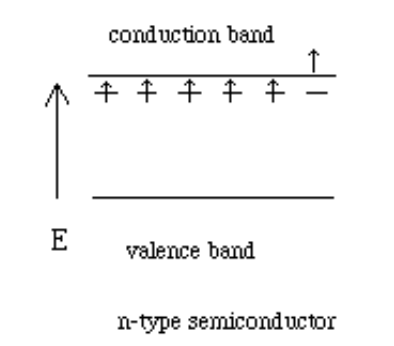
\includegraphics[width=5cm]{./images/doping.png}
		\caption{Les impuretés génèrent des niveaux d'énergie supplémentaires, ce qui nous amène à la configuration de cette figure.}
		\label{doping}
	\end{center}
\end{figure}

On peut ainsi expliciter les mécanismes qui nous amènent à observer ces trois régimes pendant qu'on augmente la température : 
\begin{description}
\item[Température très basse (non observé) : ] Pour de très basses températures, les fluctuations thermiques n'apportent pas assez d'énergie aux électrons pour qu'ils passent dans la bande de conduction, le matériau est donc \emph{isolant}.
\item[Régime A : ] Ensuite, au fur et à mesure que la température augmente, de plus en plus d'électrons venant des impuretés peuvent acquérir suffisamment d'énergie pour passer dans la bande de conduction et donc conduire le courant, le matériau devient donc \emph{conducteur}. Il est d'autant plus conducteur que la température est grande car de plus en plus d'électrons peuvent être promus dans la bande de conduction puisque l'énergie thermique qu'ils peuvent recevoir augmente.
\item[Régime B : ] Quand tous les électrons venant des impuretés sont passés dans la bande de conduction mais que l'énergie thermique n'est pas encore suffisante pour promouvoir les électrons de la bande de valence, il n'y a pas de nouvelle contribution à la conduction quelle que soit la température. Nous observons donc un palier, et même une légère diminution de la conductivité. En effet, comme dans un métal, le taux de collision entre électrons dans la bande de conduction augmente avec la température, ce qui diminue la conductivité.
\item[Régime C : ] Enfin, quand l'énergie thermique est suffisante, les électrons de la bande de valence commencent à passer dans la bande de conduction comme dans le cas du régime A avec les impuretés. On a donc une seconde phase de croissance.
\end{description}

Les deux phases de croissance observées (A et C) suivent une loi d'Arrhénius, c'est-à-dire une loi faisant intervenir une probabilité de transition (vers la bande de conduction en l'occurence) dépendant d'une énergie d'activation (ici la moitié de l'énergie du "gap" entre les bandes considérées). On a donc une densité $n$ d'électrons dans la bande de conduction de la forme : 
\begin{equation}
	n \propto exp \left( - \frac{\Delta E}{2 k_{B} T} \right)
\end{equation}
où $\Delta E$ représente la différence d'énergie entre la bande de conduction et les niveaux d'énergie des impuretés si on considère la densité d'électrons venant des impuretés ; ou bien la différence d'énergie entre la bande de conduction et la bande de valence si on prend en compte la densité d'électrons venant de cette dernière.

Puisque la conductivité du semi-conducteur est proportionnelle à la densité d'électrons dans la bande de conduction, on obtient bien deux lois d'Arrhénius pour la conductivité tantôt pour les électrons venant des impuretés, puis pour ceux venant de la bande de valence.

Pour vérifier que ces courbes montrent bien deux croissances suivant une loi d'Arrhénius, nous avons tracé le logarithme de la conductivité en fonction de $-\frac{1}{T}$, courbe qui devrait être une droite. Nous avons donc effectué deux régressions linéaires sur les deux zones de croissance (voir Figure \ref{log}).

Nous avons éliminé certains points pour ces régressions, notamment les points à basse température qui ne semblaient pas faire partie de la zone de croissance du régime A. À partir de ces régressions, nous avons pu estimer les énergies d'activation et donc les gaps $\Delta E$. Le gap entre la bande de conduction et les niveaux d'énergie des impuretés est d'environ $\Delta E = 0.2 eV$, et le gap entre les bandes de valence et de conduction est d'environ $\Delta E = 0.7 eV$. Cette valeur est tout à fait du bon ordre de grandeur pour du silicium (voir \cite{kittel_introduction_1976}), et le gap concernant les impuretés est $3.5$ fois plus faible, ce qui paraît raisonnable.

\begin{figure}[ht]
  \begin{center}
		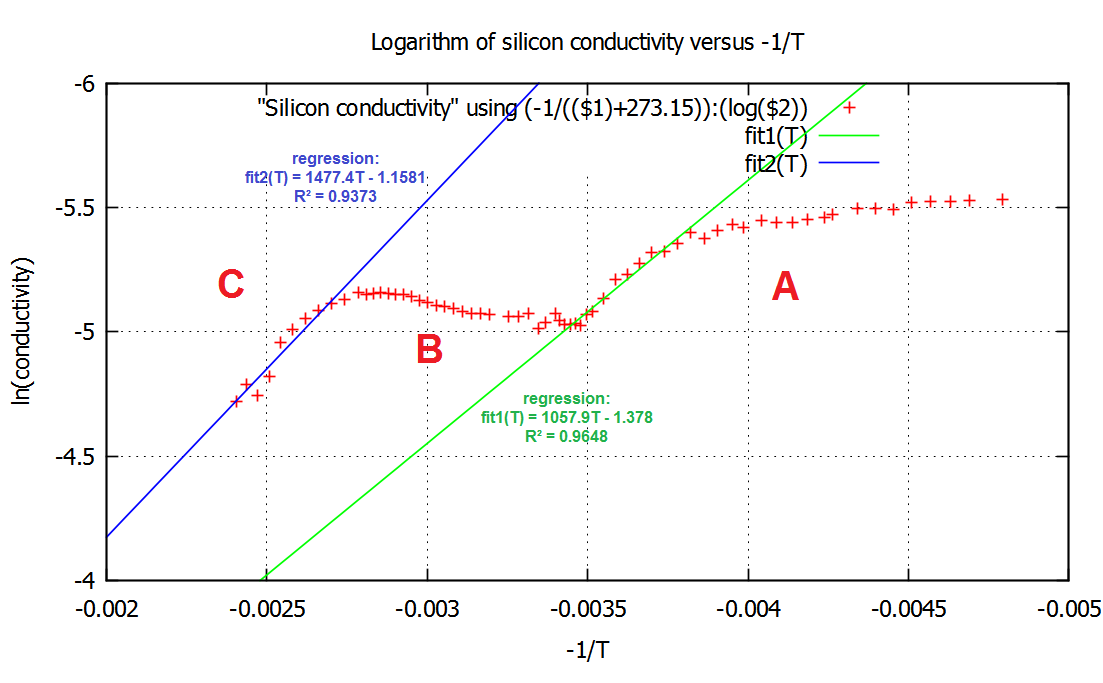
\includegraphics[width=11cm]{./images/Fit_de_log(sigma)_versus_-inverse(T).png}
		\caption{Tracé de log($\sigma$) en fonction de $-\frac{1}{T}$. Deux régressions linéaires ont été effectuées sur les deux zones de croissance en loi d'Arrhénius.}
		\label{log}
	\end{center}
\end{figure}

\subsection{Conclusions}
Nous avons bien trouvé une allure de conductivité singulière pour notre échantillon de silicium dopé N. Nous avons dégagé trois régimes décrivant cette allure, qui sont tout à fait cohérents avec les phénomènes physiques en jeu. Nous avons ainsi pu déterminer un palier de conductivité entre la température ambiante et 80 \celsius{} environ.
